% Figure contract
% Core conclusion: fixed measured wiring changes movement through a fixed body interface,
% while the separate leg-timing gate remains unresolved.
% Prototype: medium 5-stage horizontal pipeline.
% Hero: the frozen VNC core and its explicit separation from the fixed motor map.
% Evidence: existing MaleCNS anatomy/connectivity assets and reported manuscript values only.
% Target print width: approximately 17.5 cm (full-width IEEE figure*); minimum text 7 pt.
% No learned or biological behavior is implied by the anatomy and robot images.

\documentclass[tikz,border=2pt]{standalone}
\usepackage[T1]{fontenc}
\usepackage{graphicx}
\usepackage{xcolor}
\usetikzlibrary{arrows.meta,bending,calc,backgrounds,positioning}

\definecolor{ink}{HTML}{233747}
\definecolor{blue}{HTML}{256B91}
\definecolor{bluebg}{HTML}{EAF2F7}
\definecolor{orange}{HTML}{B95020}
\definecolor{orangebg}{HTML}{FFF3EC}
\definecolor{purple}{HTML}{70518E}
\definecolor{purplebg}{HTML}{F3EEF8}
\definecolor{green}{HTML}{3A7D5D}
\definecolor{greenbg}{HTML}{EDF6F0}
\definecolor{grey}{HTML}{68747D}

\begin{document}
\begin{tikzpicture}[
  x=1cm,y=1cm,
  every node/.style={font=\sffamily\fontsize{8}{9.6}\selectfont,text=ink,align=center},
  stage title/.style={font=\sffamily\bfseries\fontsize{8.8}{10.2}\selectfont,
    text=white,rounded corners=2pt,inner xsep=5pt,inner ysep=3pt,
    minimum width=2.7cm},
  small/.style={font=\sffamily\fontsize{7.2}{8.6}\selectfont},
  tiny/.style={font=\sffamily\fontsize{6.6}{7.8}\selectfont},
  chip/.style={rounded corners=2pt,draw=ink!22,fill=white,line width=.45pt,
    inner xsep=3pt,inner ysep=2pt,minimum height=.45cm},
  pin/.style={inner sep=0pt,outer sep=0pt,minimum size=0pt,draw=none},
  metric/.style={rounded corners=2pt,draw=ink!20,fill=white,line width=.45pt,
    text width=2.85cm,minimum height=.72cm,inner sep=3.4pt,align=left},
  arrow/.style={-{Stealth[length=4.5pt 1.2,width'=0pt .55,sep=0pt .4]},
    line width=1pt,shorten >=2pt,shorten <=1pt},
  arrow short/.style={-{Stealth[length=3pt 1.0,width'=0pt .5,sep=0pt .3]},
    line width=.8pt,shorten >=1pt,shorten <=0pt},
  residual/.style={-{Stealth[length=4pt 1.2,width'=0pt .55]},
    line width=.8pt,densely dashed,rounded corners=4pt,shorten >=2pt,
    shorten <=1pt}
]

\path[use as bounding box] (0,-.08) rectangle (18.1,5.62);

% Title and five equally weighted stages.
\node[anchor=west,font=\sffamily\bfseries\fontsize{10}{11.5}\selectfont,text=orange]
  at (0.05,5.39) {Measured wiring to a non-fly body};
\draw[draw=blue!35,fill=bluebg,rounded corners=4pt,line width=.65pt]
  (0,0) rectangle (3.25,5.0);
\draw[draw=orange!55,fill=orangebg,rounded corners=4pt,line width=.75pt]
  (3.55,0) rectangle (7.2,5.0);
\draw[draw=orange!55,fill=orangebg,rounded corners=4pt,line width=.75pt]
  (7.5,0) rectangle (10.65,5.0);
\draw[draw=blue!35,fill=bluebg,rounded corners=4pt,line width=.65pt]
  (10.95,0) rectangle (14.25,5.0);
\draw[draw=green!45,fill=greenbg,rounded corners=4pt,line width=.65pt]
  (14.55,0) rectangle (18.1,5.0);

\node[stage title,fill=blue] at (1.625,4.76) {Anatomy};
\node[stage title,fill=orange] at (5.375,4.76) {1. Freeze VNC};
\node[stage title,fill=orange] at (9.075,4.76) {2. Map signals};
\node[stage title,fill=blue] at (12.6,4.76) {3. Simulate};
\node[stage title,fill=green] at (16.325,4.76) {4. Evaluate};

% Stage 0: anatomy is context; the selected experiment is VNC-centered.
\node at (1.10,2.72)
  {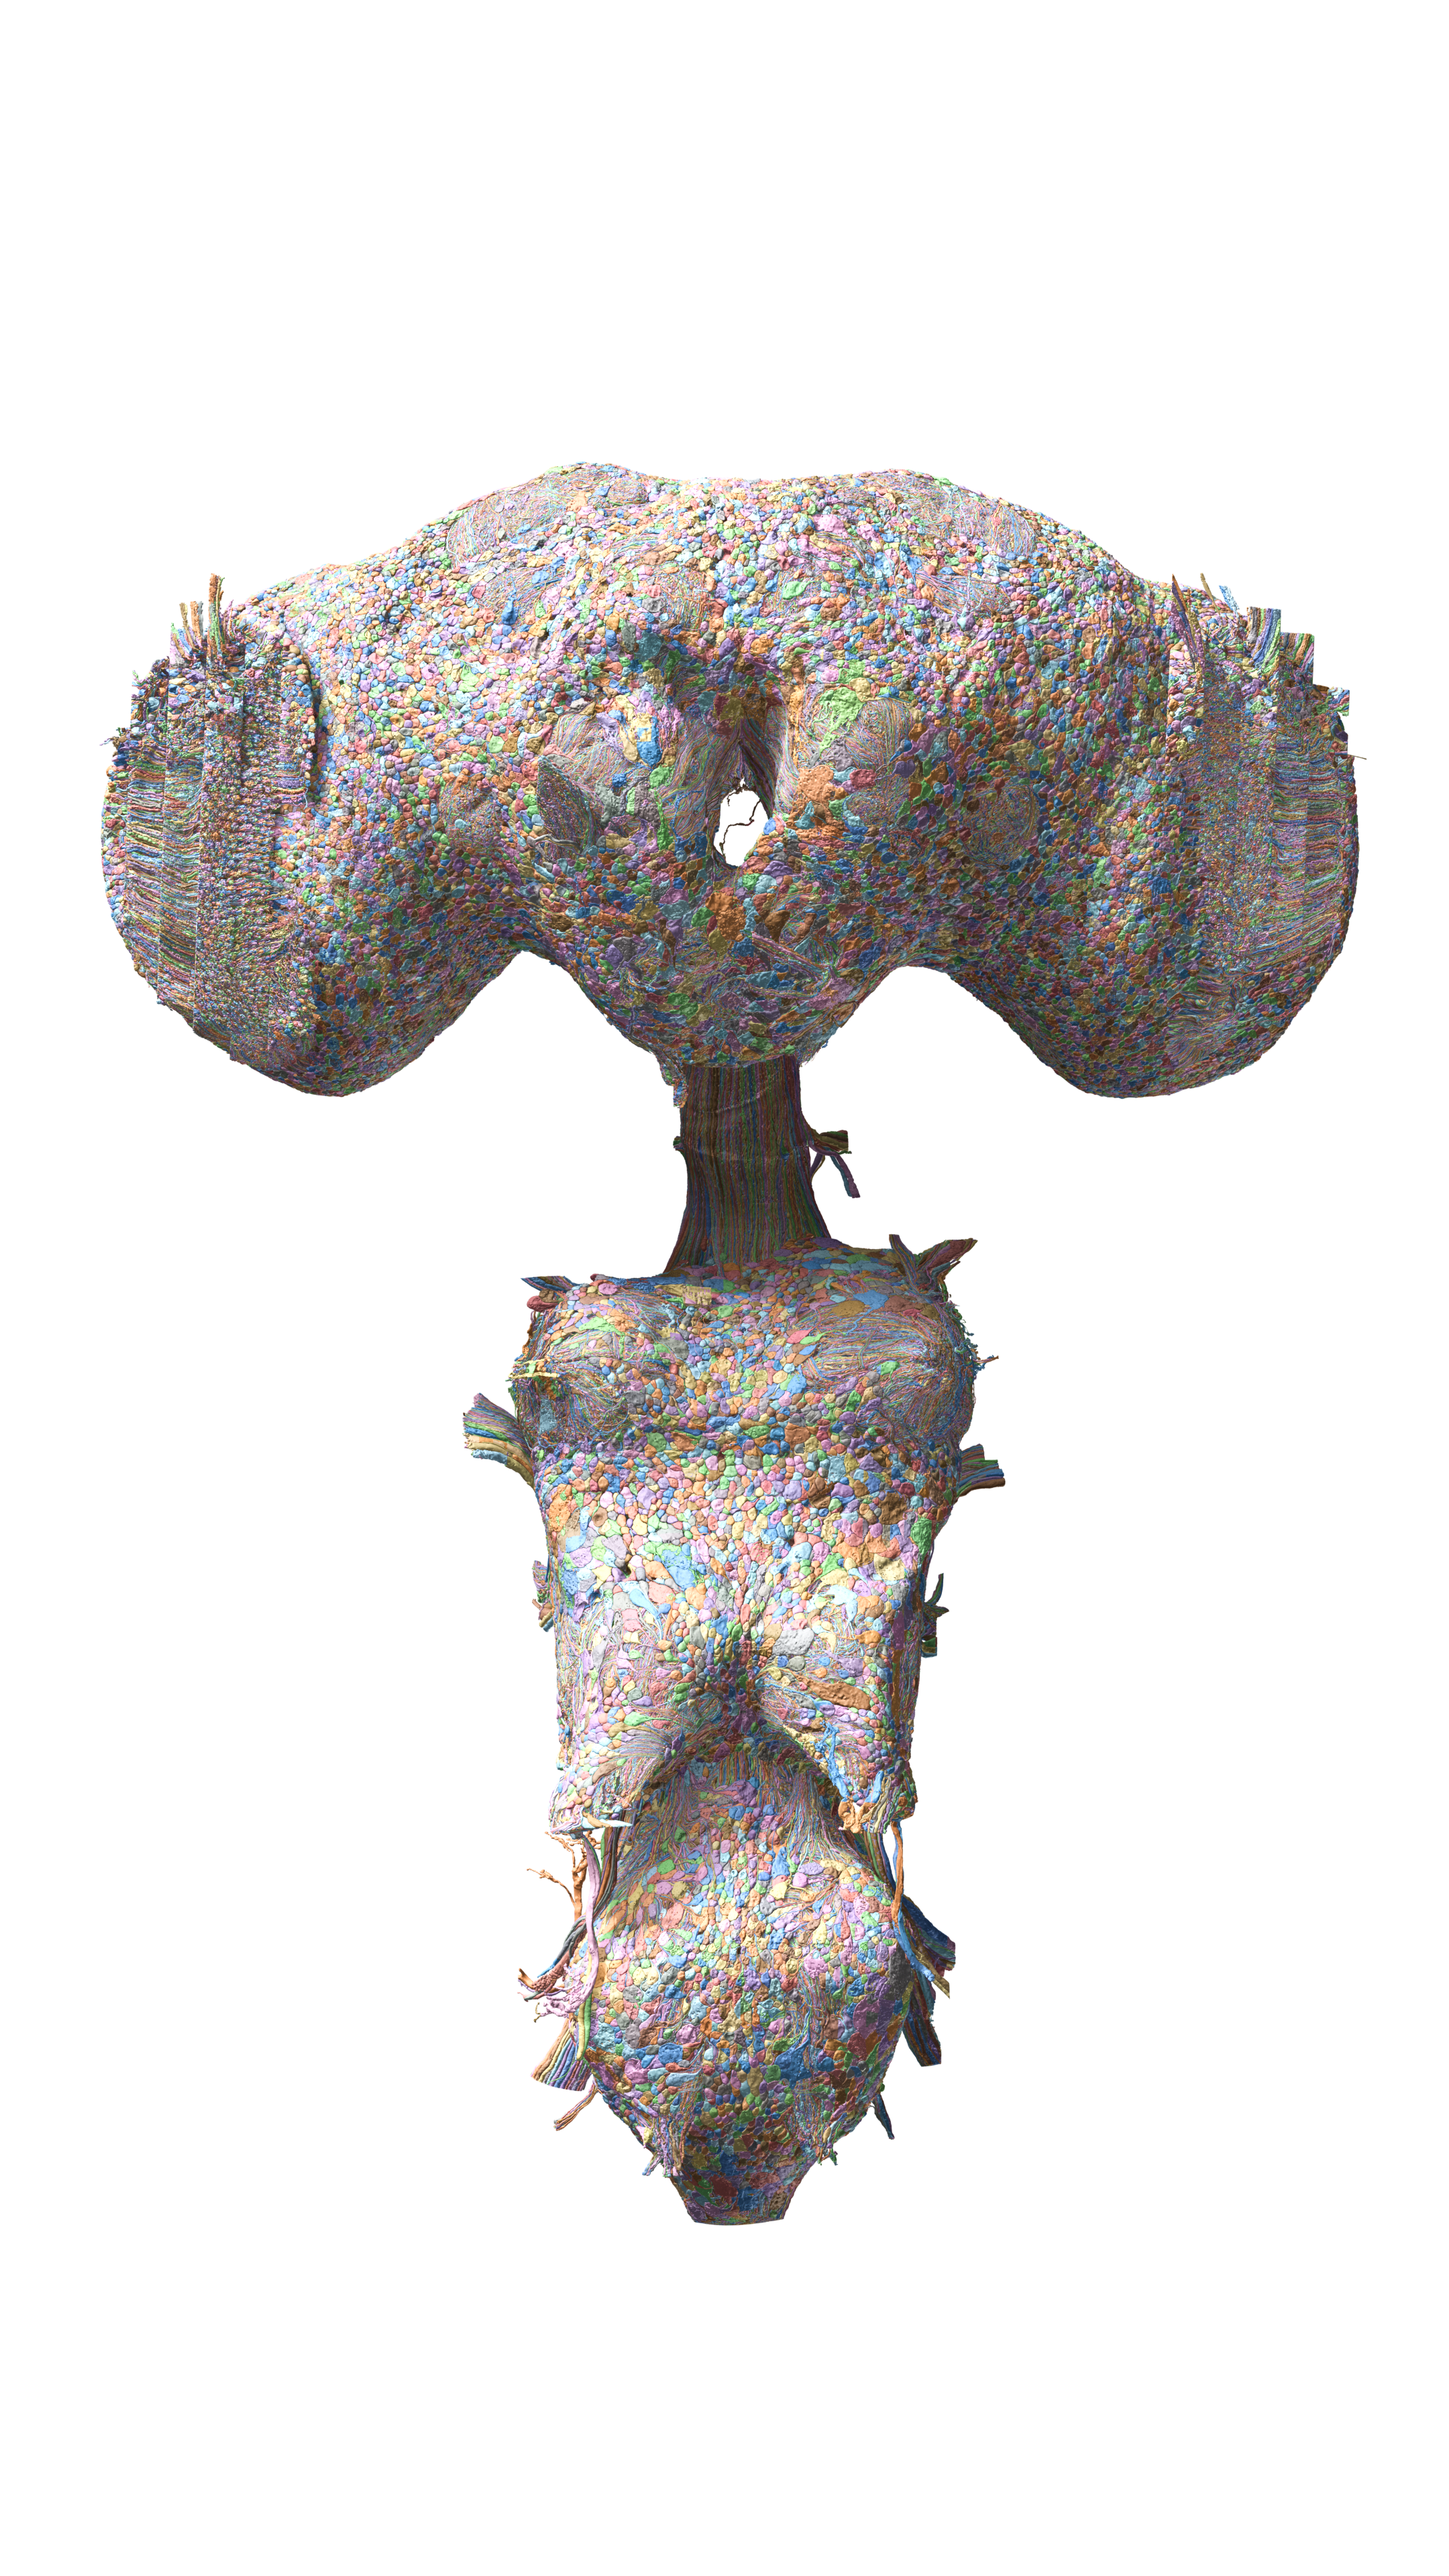
\includegraphics[height=3.05cm,trim=120 470 100 640,clip]{fly_brain_vnc.png}};
\node[small,anchor=west,fill=white,fill opacity=.72,text opacity=1,
  inner sep=1.2pt,rounded corners=1pt] at (1.72,3.87) {brain};
\node[small,anchor=west,text=orange,fill=white,fill opacity=.72,text opacity=1,
  inner sep=1.2pt,rounded corners=1pt] at (1.55,2.12) {selected VNC};
\node[tiny,text=grey] at (1.63,.28) {MaleCNS / VNC context};

% Stage 1: the connectome is the hero object.
\node[small,text=orange,text width=3.15cm] at (5.375,4.12)
  {11,000 model nodes\\[1pt]485,074 signed edges};
\node at (5.375,3.13)
  {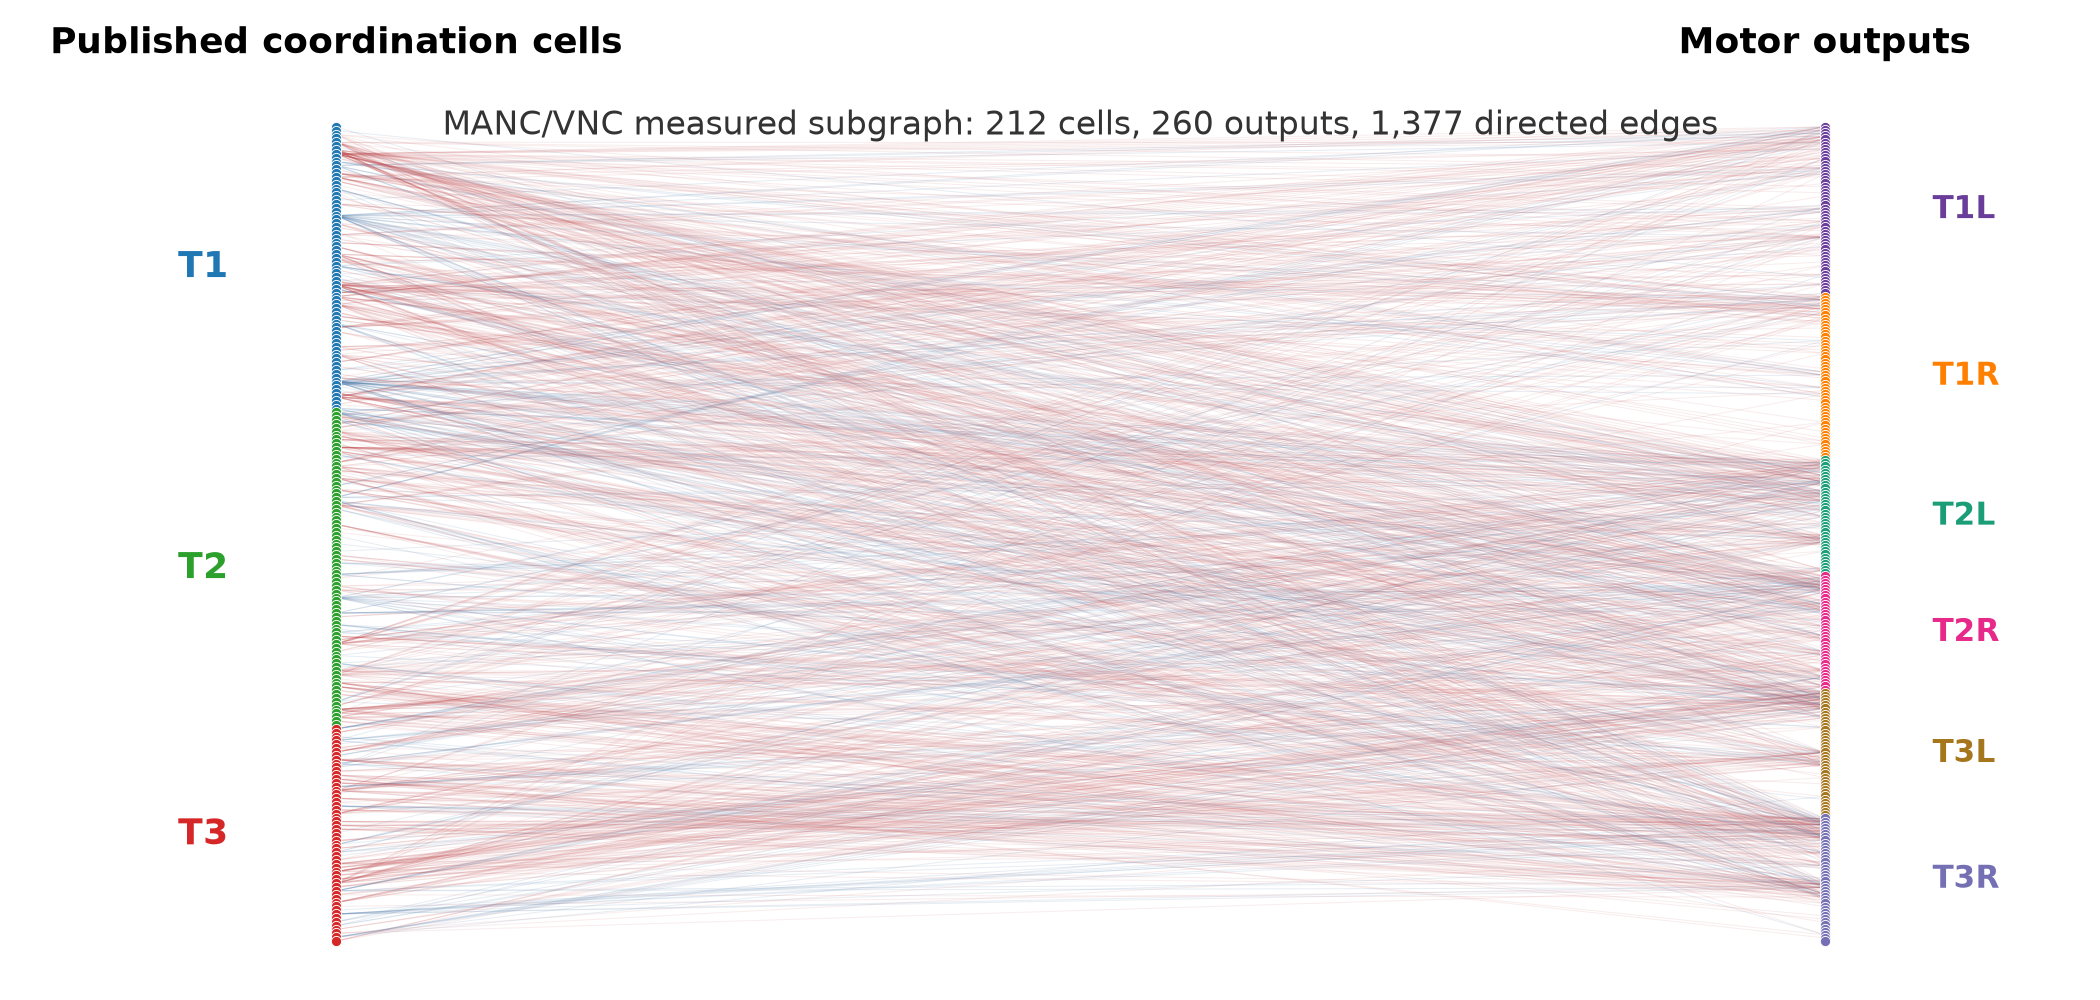
\includegraphics[width=3.16cm,height=1.43cm,keepaspectratio]{manc_connectome_context.png}};
\node[chip,minimum width=1.45cm] at (4.5,1.30) {filter $\geq 5$};
\node[chip,minimum width=1.47cm] at (6.25,1.30) {signed edges};
\node[small,text=orange] at (5.375,.65) {named descending-input drive};
\node[small,font=\sffamily\bfseries\fontsize{7.2}{8.6}\selectfont,text=orange]
  at (5.375,.30) {weights stay fixed};

% Stage 2: explicit fixed conversion.
\node[chip,minimum width=2.2cm] (signals) at (9.075,4.08)
  {260 motor channels};
\node[chip,minimum width=2.2cm] (combine) at (9.075,2.76)
  {combine opposing signals};
\node[chip,minimum width=2.2cm] (targets) at (9.075,1.44)
  {18 joint targets};
\draw[arrow short,draw=orange] (signals.south) -- (combine.north);
\draw[arrow short,draw=orange] (combine.south) -- (targets.north);
\node[small,text=orange] at (9.075,.66) {fixed map};
\node[tiny,text=grey] at (9.075,.30) {no learned conversion};

% Stage 3: actual simulator model, not an anatomical fly body.
\node at (12.6,2.88)
  {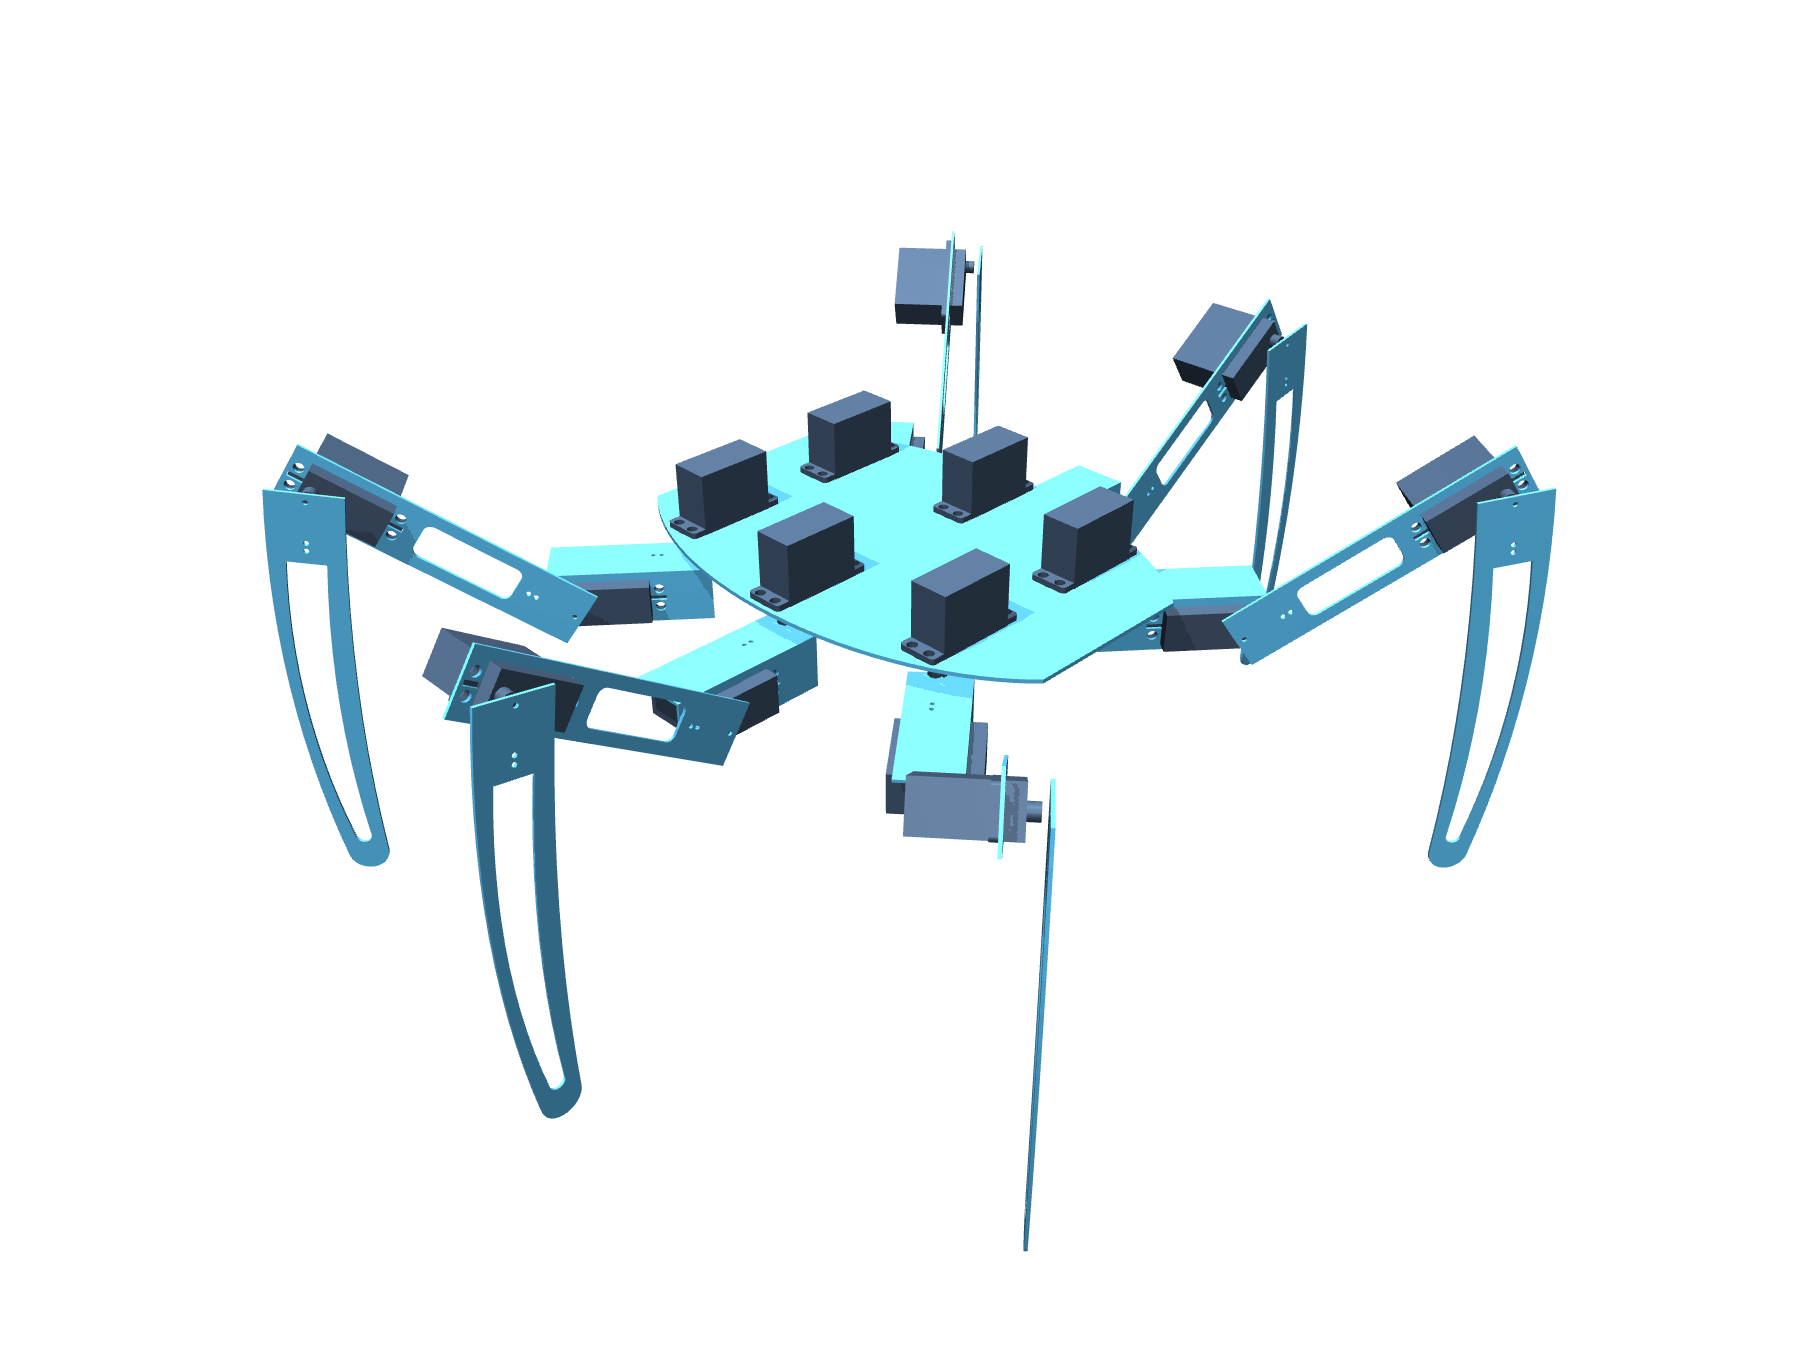
\includegraphics[width=3.05cm,height=3.05cm,trim=200 60 200 200,clip,keepaspectratio]{hexapod_model.png}};
\node[small,text=grey] at (12.6,.66) {MuJoCo  |  6 legs  |  18 joints};
\node[tiny,text=grey] at (12.6,.30) {home pose; PD joint control};

% Stage 4: outcomes are separated rather than collapsed into "walking".
\node[metric] (move) at (16.325,4.08)
  {{\bfseries\color{blue}Localized}\hfill $-$0.0112 m\\[-1.5pt]{\tiny T2 segment lesion}};
\node[metric] (turn) at (16.325,2.76)
  {{\bfseries\color{blue}Graded}\hfill $\rho=-0.886$\\[-1.5pt]{\tiny 6 rewiring fractions}};
\node[metric] (phase) at (16.325,1.44)
  {{\bfseries\color{blue}Across nine body tests}\\[-1.5pt]{\tiny 0 of 12 controls beat it}};
\node[tiny,text=grey] at (16.325,.30) {drive contrasts; gait from CPG};

% Main dataflow: short arrows only because stage gaps are under 1.5 cm.
% Invisible named anchors keep every arrow tip attached to a node boundary.
\node[pin] (flow12out) at (3.25,2.76) {};
\node[pin] (flow12in)  at (3.55,2.76) {};
\node[pin] (flow23out) at (7.2,2.76) {};
\node[pin] (flow23in)  at (7.5,2.76) {};
\node[pin] (flow34out) at (10.65,2.76) {};
\node[pin] (flow34in)  at (10.95,2.76) {};
\node[pin] (flow45out) at (14.25,2.76) {};
\node[pin] (flow45in)  at (14.55,2.76) {};
\draw[arrow short,draw=orange] (flow12out.east) -- (flow12in.west);
\draw[arrow short,draw=orange] (flow23out.east) -- (flow23in.west);
\draw[arrow short,draw=orange] (flow34out.east) -- (flow34in.west);
\draw[arrow short,draw=orange] (flow45out.east) -- (flow45in.west);

\end{tikzpicture}
\end{document}
